\section{Aims and Objectives}

The aim of this project is to develop and deploy a prototype IoT architecture with the purpose of collecting data relevant to the health of the Griffith footbridge. This involves implementing the first five layers of the architecture which consist of the coding layer, perception layer, network layer, middle-ware layer and application layer. This deployment will be achieved through the testing and implementation of two prototypes.

The first prototype is designed for testing the software and the first three layers of the IoT architecture. Two Arduino MKRWAN 1300 devices will be used, one acting as the LoRa node (layer one and two) and the other acting as a pseudo LoRaWAN gateway (layer three). The first MKRWAN 1300 is equipped with an ADXL335 3-axis accelerometer and is placed on a metal beam. The beam is vibrated along the z-axis and the device samples the acceleration. The device finds the maximum frequency peak and maximum acceleration and transmits the data via a LoRa packet. The second device receives the LoRa packet and logs the data via a serial connection. The high level system diagram in figure \ref{Proto1HLSD} presents the desired implementation of this prototype. 

\begin{figure}[h]
	\centering
	\caption{Prototype 1 High Level System Diagram}
	\label{Proto1HLSD}
	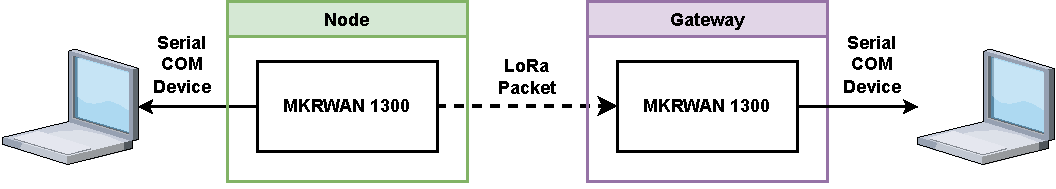
\includegraphics[scale=1]{Sections/Introduction/Prototype-1-High-Level.drawio.pdf}
\end{figure}

		The second prototype is designed for testing the software, PCB, enclosure and first five layers of the IoT architecture. The two MKRWAN 1300 devices are now both nodes and are implemented onto a custom designed PCB. This PCB is enclosed in a custom 3D printed enclosure and sits behind the guard rail of the Griffith foot bridge. The two nodes sample the maximum frequency and maximum acceleration of the bridge and transmit this data via LoRa packets to a Wisgate Edge Lite 2 LoRaWAN gateway. This gateway uploads the data via WIFI or Ethernet to the TNN cloud which acts as the middle-ware layer. --- APPLICATION LAYER WHAT IS THE IMPLEMENTATION --- Figure \ref{Proto2HLSD}
displays the high level system diagram for the second prototype. 

\begin{figure}[h] 
	\centering
	\caption{Prototype 2 High Level System Diagram}
	\label{Proto2HLSD}
	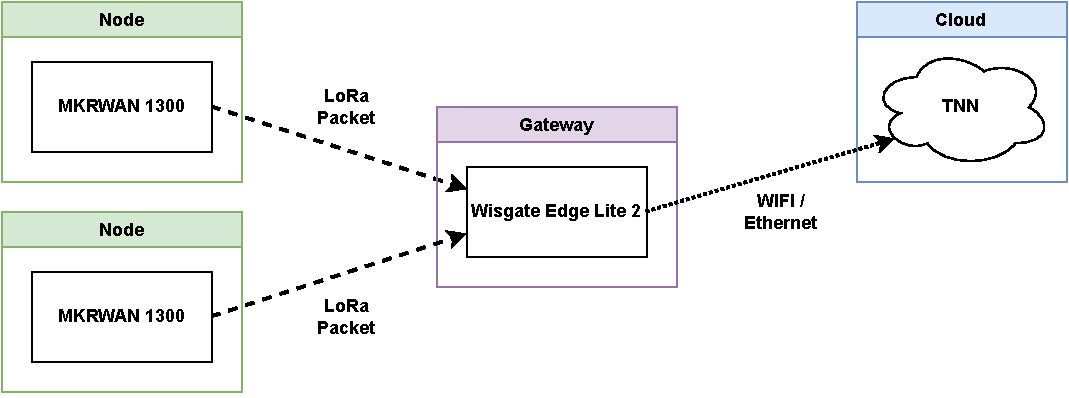
\includegraphics[scale=0.8]{Sections/Introduction/Prototype-2-High-Level.drawio.pdf}
\end{figure}

--- WHAT IS THE SUCCESS CRITERIA. SUCCESSFUL WHEN ??? ---
